\documentclass[conference]{IEEEtran}
\IEEEoverridecommandlockouts
% The preceding line is only needed to identify funding in the first footnote. If that is unneeded, please comment it out.
\usepackage{cite}
\usepackage{hyperref}
\usepackage{amsmath,amssymb,amsfonts}
\usepackage{algorithmic}
\usepackage{graphicx}
\usepackage{textcomp}

\usepackage[table]{xcolor}
\usepackage{tikz}
\usetikzlibrary{positioning, shapes.geometric, fit}
\usepackage{siunitx}
\usepackage{soul}
\usepackage{listings}
\def\BibTeX{{\rm B\kern-.05em{\sc i\kern-.025em b}\kern-.08em
    T\kern-.1667em\lower.7ex\hbox{E}\kern-.125emX}}

\usepackage[T1]{fontenc}
% T1 fonts will be used to generate the final print and online PDFs,
% so please use T1 fonts in your manuscript whenever possible.
% Other font encodings may result in incorrect characters.
%
\usepackage{graphicx}
\usepackage{hyperref}
\usepackage{amsmath}
\usepackage{amssymb}
\usepackage{mathtools}
\usepackage{bm}
\usepackage{amsfonts}
\usepackage{gensymb}
% \usepackage[caption=false]{subfig}
\usepackage{subcaption}
\usepackage[obeyFinal]{todonotes}
\usepackage[capitalise]{cleveref}
\usepackage{paralist}
\usepackage{multirow}
\usepackage{multicol}
\usepackage{float}
\usepackage{comment}

\begin{document}
\newcommand{\simon}[1]{\textcolor{red}{Simon: #1}}
\newcommand{\claudio}[1]{\textcolor{purple}{Claudio: #1}}
\newcommand{\prasad}[1]{\textcolor{green}{Prasad: #1}}
\newcommand{\lars}[1]{\textcolor{orange}{Lars: #1}}
\newcommand{\morten}[1]{\textcolor{blue}{Morten: #1}}
\newcommand{\thomas}[1]{\textcolor{brown}{Thomas: #1}}
\newcommand{\alberto}[1]{\textcolor{teal}{Alberto: #1}}
\newcommand{\carlos}[1]{\textcolor{violet}{Carlos: #1}}

% \renewcommand{\simon}[1]{}
% \renewcommand{\claudio}[1]{}
% \renewcommand{\prasad}[1]{}
% \renewcommand{\lars}[1]{}
% \renewcommand{\morten}[1]{}
% \renewcommand{\thomas}[1]{}
% \renewcommand{\alberto}[1]{}
% \renewcommand{\carlos}[1]{}

\newcommand{\methodone}{Reusable Monitor} % Other terms being considered: Monitor instance, reusable tool (old)
\newcommand{\methodtwo}{Internal Service}
\newcommand{\methodthree}{External Service}

\title{Runtime Verification of Autonomous Systems utilizing Digital Twins as a Service
    \thanks{%
        The work presented here is partially supported by the RoboSAPIENS project funded by the European Commission's Horizon Europe programme under grant agreement number 101133807, the O5G-N-IoT project, funded by the German Federal Ministry for Economic Affairs and Climate Action, due to a resolution of the German Bundestag,  % O5G-N-IoT corresponds to Iven, Leucker and Vosteen from Lübeck 
        and the SM4RTENANCE project under grant no. 101123423. % Eduard
    }
}

\author{
\IEEEauthorblockN{Morten~Haahr~Kristensen\IEEEauthorrefmark{1},
Alberto~Bonizzi\IEEEauthorrefmark{2},
Cl\'{a}udio~Gomes\IEEEauthorrefmark{1},
Simon~Thrane~Hansen\IEEEauthorrefmark{3},
Carlos~Isasa\IEEEauthorrefmark{1},\\
Hannes~Iven\IEEEauthorrefmark{4},
Eduard~Kamburjan\IEEEauthorrefmark{5},
Peter~Gorm~Larsen\IEEEauthorrefmark{1},
Martin~Leucker\IEEEauthorrefmark{4},
Prasad~Talasila\IEEEauthorrefmark{1},\\
Valdemar~Trøjgård~Tang\IEEEauthorrefmark{1},
Stefano~Tonetta\IEEEauthorrefmark{2},
Lars~B.~Vosteen\IEEEauthorrefmark{4},
Thomas~Wright\IEEEauthorrefmark{1}}
\IEEEauthorblockA{\IEEEauthorrefmark{1}\textit{Department of Electrical and Computer Engineering} \\
    \textit{Aarhus University, Denmark}\\
    \{mhk, claudio.gomes, cisasa, pgl, prasad.talasila, valdemar.tang, thomas.wright\}@ece.au.dk}
\IEEEauthorblockA{\IEEEauthorrefmark{2}\textit{Fondazione Bruno Kessler, Italy} \\
    \{bonizzi,tonettas\}@fbk.eu}
\IEEEauthorblockA{\IEEEauthorrefmark{3}\textit{Interdisciplinary Centre for Security, Reliability and Trust} \\
    \textit{University of Luxembourg}\\
    simon.hansen@uni.lu}
\IEEEauthorblockA{\IEEEauthorrefmark{4}\textit{Institute for Software Engineering and Programming Languages} \\
    \textit{Universität zu Lübeck, Germany}\\
    hannes.iven@student.uni-luebeck.de, \{leucker,vosteen\}@isp.uni-luebeck.de}
\IEEEauthorblockA{\IEEEauthorrefmark{5}\textit{Department of Informatics,  Norway,} \\
    \textit{University of Oslo, Norway}\\
    eduard@ifi.uio.no}
}

\maketitle

\begin{abstract}
    Autonomous Systems (AS) enable systems to adapt to drastic and unprecedented environmental changes, a capability that can be enhanced through the utilization of Digital Twins (DTs).
    However, the additional capabilities of AS come at the cost of explainability, as the expanding adaptation space complicates the reasoning about the system's behavior.
    For certain types of systems, it is crucial to ensure that specific properties are upheld despite the system's autonomous behavior.
    To facilitate the monitoring of these properties, we propose the use of Runtime Verification (RV).
    This tutorial demonstrates the integration of RV tools into the Digital Twins as a Service (DTaaS) platform to monitor and verify the behavior of AS in real-time.
    By exploring various methods to incorporate RV tools within a DT context, the tutorial aims to advance the application of RV technologies in autonomic computing and self-adaptive system design.
    Specifically, we demonstrate how the behavior of a self-configuring DT can be verified utilizing RV.
    This is accomplished through the DTaaS platform, which supports seamless deployment of DT-based AS.
\end{abstract}

\begin{IEEEkeywords}
    Self-adaptivity, runtime verification, digital twins, monitor, TeSSLa, NuRV
\end{IEEEkeywords}

\section{Introduction}

The vision of autonomic computing inspired new approaches to designing flexible Autonomous Systems (AS) capable of adapting to dynamic environments \cite{kephartVisionAutonomicComputing2003}.
Initially, research on AS primarily focused on reducing the complexity of large-scale software systems, which often comprise tens of millions of lines of code, particularly within purely software-based environments such as cloud computing.
Since then, the field has advanced significantly, extending its concepts to new domains including dynamic software architectures \cite{Albassam:2017:DARE}, robotics \cite{Cheng:2020:ACROS}, business process management \cite{malburgApplyingMAPEKControl2023}, and cyber-security \cite{Papamartzivanos:2019:ItrusionDetection}.
However, the adaptability of these systems presents significant challenges in ensuring that key properties of the system are consistently met.
As a concrete motivational example, within the domain of robotics, there is a critical need for flexible self-adaptive robots that can operate reliably despite dynamic environmental changes.
Nevertheless, the safety of human life must never be compromised, and ensuring that these robots adhere to safety standards despite their self-adaptivity remains an ongoing challenge.
Research addressing these challenges, such as \cite{Cheng:2020:ACROS} and \cite{jahanMAPEKMAPESACInteraction2020a}, involves formulating and validating the adherence to requirements at runtime.
Similar requirements for continuous monitoring of system properties are present in other domains utilizing AS.
Consequently, self-adaptivity can be considered as the component that increases the system's set of possible behaviors, while Runtime Verification (RV) serves as the component that ensures unwanted behaviors are excluded from this set.

The tutorial focuses on how researchers within the AS community can utilize RV tools within their work to ensure the correctness of their systems.
In doing so, emphasis is placed on the different ways that RV tools can be integrated within a deployment platform and utilized by the existing system.
Through this process, we aim that attendees will become familiar with how services are deployed, as well as gain practical insight into how to build monitoring services.
The tutorial adopts a hands-on approach, utilizing the Incubator case study \cite{Feng2021, Feng2022}, which features a Digital Twin (DT) capable of self-configuring during anomalous situations.
Although the tutorial is presented within the context of a DT, the majority of the concepts discussed extend beyond this specific application.
Through the Incubator, we explore five different scenarios for integrating an RV tool within an existing AS, all of which are deployed on the Digital Twin as a Service (DTaaS) platform (detailed in \cref{sec:background}).

The tutorial is structured as follows: \cref{sec:background} introduces the main background concepts for following the tutorial.
Then \cref{sec:examples} presents five distinct examples showcasing the implementation of monitoring using two different RV frameworks.
Finally, \cref{sec:conclude} provides a few concluding remarks about the tutorial.
%
\section{Background}\label{sec:background}

\subsection{Runtime Verification}
RV is a lightweight method of improving the integrity of deployed systems, and focuses on augmenting a system with additional monitoring functionality, in order to avoid unintended behavior at runtime.
This is accomplished through a variety of monitoring techniques, which check whether a system conforms to specifications based on traces or streams of data from the running system.

A wide range of RV methods have been developed over the years, offering a variety of different specification languages for expressing the desired behavior of the system including temporal logics such as Linear Temporal Logic (LTL)~\cite{pnueli1977ltl} and Signal Temporal Logic (STL)~\cite{donze2013stl} as well as domain-specific languages such as TeSSLa~\cite{convent2018tessla}.

RV also encompasses both passive monitoring techniques which focus on detecting errors without changing the behavior of the system, as well as more active techniques (also known as \emph{runtime enforcement}~\cite{falcone2010runtimeenforcement}) which aim to block or correct bad behaviors.

\subsection{NuRV}

NuRV~\cite{CimattiTT19a}\footnote{\url{https://nurv.fbk.eu}} is an extension of the nuXmv model checker for assumption-based LTL RV with partial observability and resets. Monitoring formulas are specified in LTL while assumptions are in SMV. Thanks to the assumption, the output of the monitor can be conclusive also if the formula contains future operators or if not all variables are observable.

The tool provides commands for online/offline monitoring and code generation into standalone monitor code. Using the online/offline monitor, LTL properties can be verified incrementally on finite traces from the system under scrutiny. The code generation currently supports C, C++, Common Lisp, and Java, and is extensible. Furthermore, from the same internal monitor automaton, the monitor can be generated into SMV modules, whose characteristics can be verified by Model Checking using nuXmv.

\subsection{TeSSLa}
The Temporal Stream-based Specification Language (TeSSLa)~\cite{convent2018tessla} framework\footnote{\url{https://tessla.io}} combines a language and a suite of tools designed for real-time verification of systems through data stream analysis. TeSSLa allows the declaration of input data types and the transformation of this data into new, derived streams by applying a series of defined operations. This approach enables effective monitoring of complex systems, ensuring accurate tracking and analysis without overly complex processes.

TeSSLa provides extensive libraries and supports the creation of macros. These macros allow users to define custom operations, simplifying the specification of complex behaviors and increasing the accessibility of the language. TeSSLa also supports the generation of detailed output streams, including statistical data with precise event timestamps, and allows integration with monitoring tools developed in modern programming languages such as Rust and Scala. Its integration with the metrics collection agent Telegraf~\cite{TT-Connector} contributes to its effectiveness in real-world applications.
At its core, TeSSLa's strength lies in its ability to map input data to meaningful outputs, which is essential for real-time system monitoring and informed decision-making in areas such as DT technologies.

\subsection{Digital Twins as a Service}
The DTaaS\footnote{\url{https://github.com/INTO-CPS-Association/DTaaS}} platform is a collaborative platform to build, use, and share DTs.
It is based-off a microservices architecture with dedicated software containers\footnote{Container is a software component at level-2 of the C4 model.} for DT assets, user workspaces, platform services, a front-end website, and service router.

One of the architectural principles used in the development of DTaaS is to conceive DTs as composed of reusable assets, which separate the functionality into their constituent parts.
Within DTaaS, data, models~\cite{Zambrano&22}, tools~\cite{qi2021enabling}, services~\cite{budiardjo2021digital,robles2023opentwins} and ready to use DTs~\cite{aziz2023distributed} have been identified as reusable assets.
The DT Assets software container provides an interface to perform create, reuse, update, and delete operations on the reusable stored within the DTaaS.

Users utilizing DTaaS have private workspaces in which they can build and use systems, from where they can access assets as a regular part of the filesystem.
All workspaces have internet access thereby enabling the integration of DTs running inside workspaces with external software systems.

Out-of-the-box, DTaaS supports multiple commonly used services across DTs and users.
The most commonly used are RabbitMQ and MQTT (communication), InfluxDB and MongoDB (data storage), and Grafana (data visualization).
Additionally, it is possible to host private services accessible to a selected number of users.
These services include the run-time services provided by TeSSLa and NuRV.

\subsection{FMI-based Co-simulation}
\label{sc:fmi}
Integrating verification methods early in development ensures system correctness from the start \cite{Prasad&21a}.
One approach is \textit{co-simulation}, which combines multiple simulation tools into a single simulation~\cite{Gomes2018,Kubler2000}.
Co-simulation is crucial for modeling complex systems co-developed by multiple organizations and systems whose complexity transcends the capabilities of any single simulation tool.

Interoperability between heterogeneous simulation tools is achieved using Functional Mock-up Units (FMUs) defined by the Functional Mock-up Interface (FMI) standard~\cite{FMI2014}.
An FMU encapsulates the behavior of a \emph{dynamic system}, whose state evolves according to \emph{evolution rules} and \emph{external stimuli}, into a discrete trajectory.
This allows complex behaviors to be represented modularly while protecting intellectual property.

Multiple FMUs are composed into a \emph{scenario} by coupling their input and output ports to represent the behavior of a complex system.
A \emph{coupling} signifies that the state of one FMU (the output) directly influences the state of another (the input).
A scenario is simulated using a co-simulation framework that interacts with the FMUs through their interface to advance them in lockstep and exchange values between the coupled ports.
%
% \section{Methodology}\label{sec:methodology}
Integrating RV with AS requires connecting the concrete AS \textit{instance} with the concrete RV monitor instance(s).
These instances must be generated, managed, and linked within the platform, DTaaS, throughout their lifetime.
Consequently, AS researchers must understand the various approaches available for integrating the RV monitors.
In this section, we present different methods for integrating the monitors into AS.

\subsection{The Digital Twin Assets and Lifecycle Phases}
\label{sec:dt-integration}

Each DT asset, that is managed inside DTaaS, is a reusable component falling into one of the following categories:

\textbf{Data:} a DT asset that provides data from the PT (a data source) or consumes data (a data sink) from a DT. The data asset can have its origins in two different places. The first source of data is PT which can either be a real one, or a mock. The mock PTs help with the DT development. The second source of data is the environment in which PT operates. Similar to PT, the environment data can come from sensing the environment around PT or a mock version of the environment.

\textbf{Model:} describes the physical behavior of the PT. The models can be physics-based, numerical, data-driven, co-simulation, or a combination thereof. Both PT and DT will have their models. While the PT models are used for product development, DT models are used for instantiating digital replicas of the PT. It is advantageous to use the same model for both PT and DT but is often not possible primarily due to: 1) the lack of availability of the same model among all users, 2) divergent technical needs needing different models, 3) modeling software not being able to create models usable inside DTs.

\textbf{Tool:} a software tool that can be used to create, evaluate, and analyze a model. Tools tend to be more reusable than models. For example, software tools such as Matlab\footnote{\url{https://mathworks.com}} can generate and evaluate models of different types (physics, numerical, co-simulation, etc.). The tools can also be used to perform in-time generation of models. In this case, the actual DT models are generated from a model configuration file when the DT is about to be executed. Some of the RV tools fit into this category because these RV tools generate monitoring at the start of executing DT.

\textbf{Service:} provides a well-defined functionality over inter-process communication or computer network. Each service runs as one or more operating system processes accessible over an application programming interface (API). A service is reusable by all eligible consumers of that service. Within the context of DTs, services are used to satisfy concurrency and external integration needs. A DT performing run-time monitoring might send alerts to users or other external services (such as quality control audit software).

%
\begin{figure}[]
	\centering
	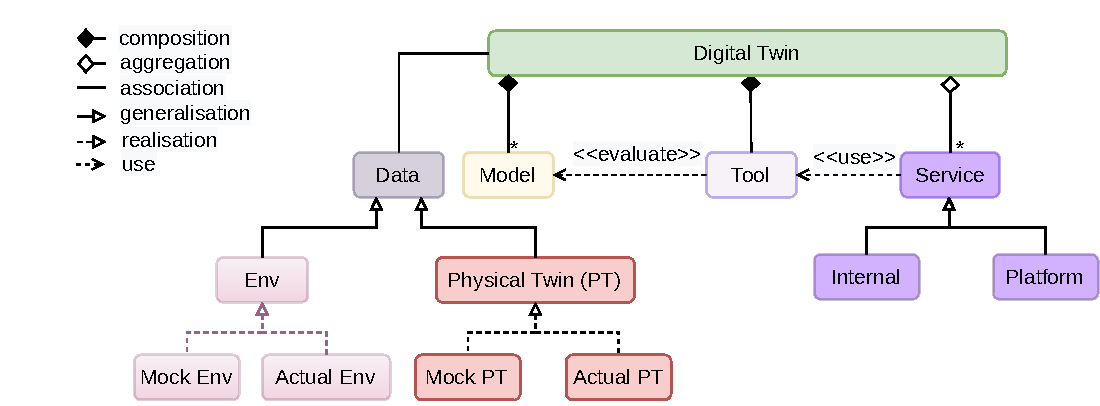
\includegraphics[width=\columnwidth]{images/assets-relationship.pdf}
	\caption{A class diagram for DT. The diagram illustrates the composition of data, models, tools, and services to form a DT. \morten{Consider if needed}}
	\label{fig:dt-class-diagram}
\end{figure}%
%
\cref{fig:dt-class-diagram} shows a class diagram of DT. The four types of reusable assets - data, models, tools, and services - are shown as separate classes. Each class has properties that need to be defined at the DT instantiation time. For example, a data source conforming to MQTT protocol needs to have the MQTT broker access details. Here the access details are the properties of the data class. Similarly, models might have initial values, services will have service definitions/configurations and tools will have configurations. The DTaaS platform provides templates for supplying properties to DT and all assets used in it. A DT asset provider needs to provide the configuration template in which the properties can be filled.
The DT creator creates a DT-level configuration template and creates a configuration program/script whose primary responsibility is to translate the top-level DT class properties (configuration values) to asset-level properties. The DT users update the configuration values to create DT instances and link them with PTs.
The RV tool providers need to provide configuration templates for their RV tools so that the DT creators can translate the DT properties to the configuration values of their RV tools.
%\morten{Perhaps, this can come earlier to follow a more top-down approach.}\prasad{Explaining RV config with explaining the need for config seems confusing. Perhaps I can use example configs from section 4 in a table to illustrate the type of configs RV providers can use.}

It is important to remember that the class relationships shown in the \cref{fig:dt-class-diagram} can follow all variations of class associations. The actual class relationships shown in the figure reflect the examples being presented in this tutorial. The DT has an association type relationship with data coming from both PT and its environment. The DT class has composition type of relationship with Model, and Tool classes. The services are only aggregated by the DT class. In the case of services that are reusable simultaneously across multiple DTs, aggregation is the most appropriate class relationship. Similarly, in the case of any assets whose instances are only used exclusively within a DT, the relationship necessarily is that of composition. The models and tools need to be instantiated uniquely for each DT and thus they both tend to have composition type relationship with their DTs.
In addition, there is also a dependency relationship between the assets themselves, especially among services and tools. Some tools can also be run as services which will be showcased in the examples below.

A PT goes through multiple lifecycle phases necessitating the support for lifecycle phases within DTs. Certain research communities use design-manufacture-operate-recycle phases as representative lifecycle phases for a PT. This tutorial illustrates the use of RV tools on DTs during the operational phase. Thus only the \emph{create}, \emph{execute} and \emph{terminate} lifecycle phases are being illustrated. Two different kinds of activities are undertaken in the create phase: 1) creation of models, monitors if any 2) creation of execution environment by installing the necessary dependencies.
The execution phase includes the instantiation of DT and its use. The DT is available for interaction and the monitors are active in this phase. Finally, the terminate phase includes the termination of DT execution and revocation of all resources allocated to the terminated DT.

\subsection{General Techniques for Monitor Integration}
Several approaches exist for integrating RV monitors into DTs, dependent upon the capabilities of the underlying RV tool.%\prasad{Only the NuRV generates monitors. The TeSSLa takes monitoring properties and works as is without generating a separate monitor.}
Consequently, certain monitors may offer greater flexibility and require less effort to integrate from the perspective of DT developers.
Regardless of the approach, a monitor instance must be established and linked to each twin instance (DT asset) for monitoring individual properties.
The differentiating factor lies in whether the monitor is exposed as a service and who manages its lifecycle.
We distinguish the following approaches:

\textbf{\methodone:} The RV tool, below just called ``tool'', is published as a reusable asset for the platform that generates a monitor instance used within a twin instance. The tool merely generates the monitor instance, which afterward is completely inside the twin instance, meaning their life cycles are tied together.

\textbf{\methodtwo:} The tool is published as a reusable service that is instantiated from a twin instance.
Each twin instance manages its monitor instance as an internal service.

\textbf{\methodthree:} The tool is published as a reusable service that is instantiated and managed outside of twin instances.
The twin instance uses it as an external service.
When the twin instance finishes, the monitor service continues to be active. Any future twin instances can reuse the same external service.

In the following, we describe each possibility in detail before providing a guide on deciding which approach to take.

\subsubsection{Runtime Verification as a \methodone}
In this scenario, the RV tool is invoked to generate the monitor when the twin instance is created -- once for each property that the twin instance requires to be monitored.
Each invocation creates one reusable monitor, which is packaged as a binary, for example, a Functional Mock-Up Unit.
The binary is then sent to the twin instance -- it is the task of the twin instance to integrate the monitor instance into its application.

As a consequence, the platform itself is unaware of the monitor instance -- it is handled completely within the twin instance -- which makes this option the most lightweight when it comes
to extending the platform. Concerning the twin instance itself, however, it requires a tight coupling between the platform tool and monitor instance --
changing the application may require changing the platform tool.
Similarly, as the platform is unaware of the monitor instance, it must be handled by the twin instance during shutdown.
In particular, its results, e.g., violation logs, must be stored.

%You are right about the mix-up of terms. I made the mistake of not labeling the DT assets correctly. We should use the following DT assets:
%Data, Models, Tools, Functions and Services
%
%The patterns may be explained as follows.
%
%    RV is published as a reusable tool takes a model input and generates a model used to be used within DT. In this, a model asset is converted to another model just-in-time and then DT is run. NuRV is an example of this scenario.
%    RV is published as a reusable service and is used inside DT as a service. I think we can keep RVs as services and then integrate them into DT. The service remains active only when the DT is active. Tessla as implemented in firefighter use case is an example of this scenario.
%    RV is published as a platform service and is used inside DT as a service. In this scenario, the service is always available an active DT uses the platform service. I am told that Tessla can work in this mode but we don't have an example for this scenario.
%
%
%The second is a reuse of the following
%
%    Same RV properties used with different RV tool/service in same or different DTs. In this case, a DT configuration can select an RV tool.
%    Different RV properties are used with one RV tool/service. In this case, RV properties are specified in the DT configuration, and the RV tool runs with the selected RV property.
%
%We don't have examples of this kind of reuse.
%
%The diagrams need to be corrected by changing the terms. I hope the explanation is clear.


\subsubsection{Runtime Verification as an \methodtwo}
In this scenario, the RV tool generates the monitor as an internal service, that is started and stopped alongside the twin instance.
The twin instance, once started, provides the property to the RV tool and then connects to the newly started RV service. Potential advantages are:
\begin{enumerate}
	\item decoupling of RV tool deployment
	\item possibility of defining RV properties from DTs
	\item possibility of creating multiple instances of an RV service (one per DT)
\end{enumerate}%
%
As a consequence, the twin instance manages the monitor service instance; for example, its start and shutdown must be managed in the twin instance.
The twin instance has a clear interface to interact with the internal monitor service and, thus, is potentially less tightly coupled,
as the interface can abstract away from all details except for data exchange.

\subsubsection{Runtime Verification as an \methodthree}
In this scenario, the RV monitor exists as an external service to the twin instances. This means multiple twin services can use the same monitoring service and each twin instance can interact with its coupled monitor instance through an API.
As a consequence, this approach completely decouples the twin and monitor instances, with all logic related to the monitor instance managed independently.
The twin instance continues to utilize a clear interface, while the monitor instance can be subjected to fine-grained control beyond the possibilities of general workflows within each twin instance.
However, this necessitates a separate implementation of all lifecycle management for the RV service, potentially leading to redundancy with features already present either within separate twin instances or the platform services.

%\prasad{Can the purpose be placed after the discussion?} no, the discussion is in light of the purposes
\subsubsection{Purposes}
Integrating a monitor can serve several purposes in a DT, and we briefly discuss the most relevant. The purpose must be considered when choosing the integration approach.
It is out of the scope of this tutorial to discuss all possible uses of RV, and we focus on three groups: Interaction, target structure of the monitor, and target concept of the monitor.

For interaction, the purpose of the monitor instance is to target different levels of interactions with the twin instance.
On one extreme, it may merely \emph{report}, i.e., run alongside the twin instance and output a warning or summary to the user without influencing the behavior or structure of the twin instance.
Conversely, the output of a monitor instance can be used directly to \emph{control} the PT from the twin instance.
In between, the monitor instance can act as a  shield~\cite{DBLP:conf/tacas/BloemKKW15}, i.e., manipulate the data streams between PT and DT to ensure some property without being a complete controller.

We stress that this discussion is orthogonal to the classification of a system as digital shadow or DT~\cite{KRITZINGER20181016} -- if the monitor instance is used as a reporting tool, the overall system may still be a DT, as other components may implement the control loop.

For the target structure and concept, the monitor instance is monitoring some stream of data. This can either be from the PT, i.e., monitoring sensor streams, the DT itself, i.e., monitoring control streams, or their combination, i.e., or the \emph{interconnection} between the PT and DT.

Finally, the monitor instance can monitor \emph{behavior}, or it can monitor \emph{structure}, where monitoring structure does not influence the control and data streams between the PTs and DTS, but the internal composition of the twin instance -- which may be connected to the PT via an asset model or similar~\cite{DBLP:conf/isola/KamburjanKSTCJ22}.


\subsubsection{Discussion}
RV tool providers must consider which of the approaches they wish to support with their generated monitors.
Supporting the \methodone\ approach provides a tight coupling between the monitor and twin instances, which makes this integration more accessible at the cost of manual handling of the tool lifecycle for the user.
The implementation effort for this approach is relatively low, as the tool instance only generates a binary.
Supporting the \methodtwo\ approach gives a looser coupling, which provides more flexibility (as it enforces a specific lifecycle and interface) but neither requires the user nor the DT developer to handle the lifecycle.
Supporting the \methodthree approach, in contrast to \methodtwo, gives the DT developer more flexibility, as they can improve the management of multiple monitor instances through more precise lifecycle management.

Finally, the purpose must be considered. Tight interaction, such as control, benefits from the flexibility of service integration, while loose interaction can be realized with less effort on the development side. Regarding the target, a platform service may perform some optimization if several services are using monitor instances for the same PT. Finally, structural monitoring and reconfiguration are easier to realize if the structure of the twin instance is easily available, i.e., it is a platform tool integration.

% \Cref{fig:choice} gives an overview of the trade-off without considering the purpose.
%\begin{table}[]
%\begin{tabular}{l|llll}
%                 & effort (user) & effort (integration) & flexibility (user)       & flexibility (integration) \\ \hline
%Platform Tool    & high          & low                  & high                     & low                       \\
%Reusable Serv.\ & low           & low                  & low                      & low                       \\ 
%Platform Serv.\ & low           & high                 & low & high 
%\end{tabular}
%    \caption{Overview over the flexibility-effort trade-off}
%\label{tab:choice}
%\end{table}


%\lars{a diagram like \cref{fig:choice} might be easier to grasp than a table; @Eduard do you think the reduction to two dimensions fits the problem?}\prasad{the graph is better and is an equivalent representation to table.}

% \begin{figure}
% 
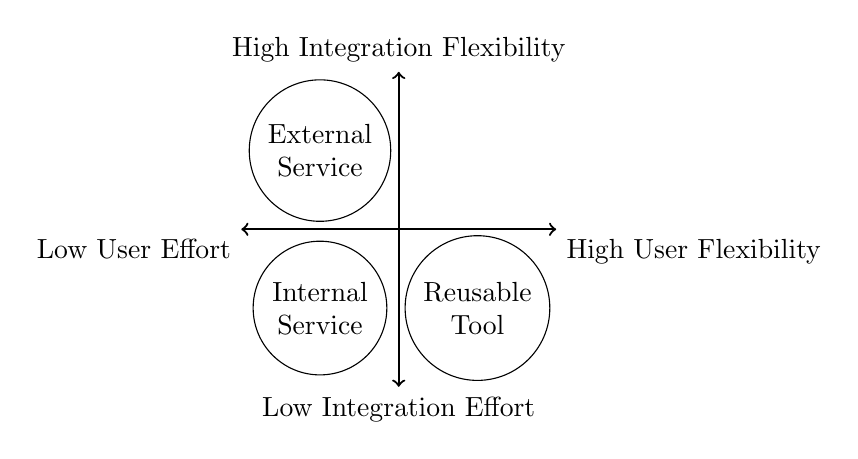
\begin{tikzpicture}[scale=1, every node/.style={scale=1}]

    % Draw axes
    \draw[thick,->] (0,0) -- (2,0) node[anchor=north west] {High User Flexibility};
    \draw[thick,->] (0,0) -- (0,2) node[anchor=south ] {High Integration Flexibility};
    \draw[thick,->] (0,0) -- (-2,0) node[anchor=north east] {Low User Effort};
    \draw[thick,->] (0,0) -- (0,-2) node[anchor=north ] {Low Integration Effort};

    % Add the three combinations
    % Reusable Service: Low Integration Effort and Low User Effort
    \node[align=center, draw, circle] (RS) at (-1,-1) {Internal\\Service};

    % Platform Tool: Low Integration Effort and High User Flexibility
    \node[align=center, draw, circle] (PT) at (1,-1) {Reusable\\Tool};

    % Platform Service: Low User Effort and High Integration Flexibility
    \node[align=center, draw, circle] (PS) at (-1,1) {External\\Service};

\end{tikzpicture}


% \caption{Overview over the flexibility-effort trade-off}
% \label{fig:choice}
% \end{figure}

%
\section{Example integrations}\label{sec:examples}

Five examples showcasing the RV integration into the AS are presented below: three utilizing NuRV and two utilizing TeSSLa.
For NuRV, the first example demonstrates a scenario where the components of a self-adaptive DT are validated before the system is deployed.
This involves exporting the NuRV specification as an FMU and conducting co-simulations with the other components of the system.
In the second example, the reusability of the FMU within a service-oriented architecture is demonstrated, enabling RV on the deployed system.
It listens to real-time sensing data sent by the Physical Twin (PT), i.e., the physical counterpart of the system, through RabbitMQ to the DT, evaluating the truth value of LTL formulas.
In the third example, the NuRV specification is deployed on a standalone server, with its services exposed to the DT.
As a result, it is uncoupled from the DT instance.
For TeSSLa, the two examples demonstrate passive and active monitoring.
In passive monitoring, an alarm is raised in the event of a violation of the monitored conditions.
In contrast, active monitoring entails altering the system's behavior if a monitored condition is falsified.
\subsection{The Incubator}
%\fbox{Budget: 0.5 page for this subsection}
The different ways of integrating RV monitors into DTs are showcased using the incubator system described in~\cite{Feng&21c}. An overview of this system can be seen at~\cref{subfig:incubator_hw} and~\cref{subfig:incubator_blocks}.
The objective of the incubator is to keep the temperature inside a box close to a target temperature, a task that can be difficult to achieve as more complexities surround the system, such as the possibility of someone opening the lid or the object inside the box releasing heat, are considered.
These considerations have led to the development of a DT for this system~\cite{Feng2022}, which consists of a dynamical model of the physical components of the PT and software components capturing its controller behavior. Additionally, the DT contains a self-adaptation service that reacts to possible changes in the environment and adjusts the incubator's objective as necessary. In order to do this, a MAPE-K architecture is implemented, where a Kalman filter estimates the state of the system and compares it to the empirical data from the sensors. As soon as a deviation is detected, the DT looks at historical data to identify the anomaly and plan accordingly.
The incubator DT has undergone previous verification work, mainly~\cite{Wright2022}, in which the authors propose using reachability analysis to verify that self-adaptations cannot lead to future unsafe states of the incubator.

The approach that we propose in this work differs in the technique used, as we use runtime monitoring to check the truth value of an STL formula that describes the desired behavior of the interaction of the services that belong to the incubator DT.
In order to enable the monitoring of the desired service interaction, a small redesign of the incubator DT architecture was needed.
The self-adaptation service was divided into two different services: anomaly detection, which handles detecting the difference between the expected temperatures and the sensed temperatures, and energy saving, which changes the target temperature to a lower one in case the anomaly detection service has detected an opening of the lid.
Additionally, a runtime monitoring service has also been implemented in the DT, ensuring the correct combined behavior of the anomaly detection and energy saver blocks.
The service monitors the following STL property:
\begin{equation}
	\square(A\implies \lozenge_{[0,3]} S)
\end{equation}
where $A$ stands for the anomaly detection service detecting the opening of the lid and $S$ stands for the energy saver service changing the target temperature. An overview of the interaction of these services and the PT can be seen at~\cref{subfig:incubator_anomaly}.

\begin{figure}[ht]
	\centering
	\begin{subfigure}[t]{0.48\textwidth}
		\centering
		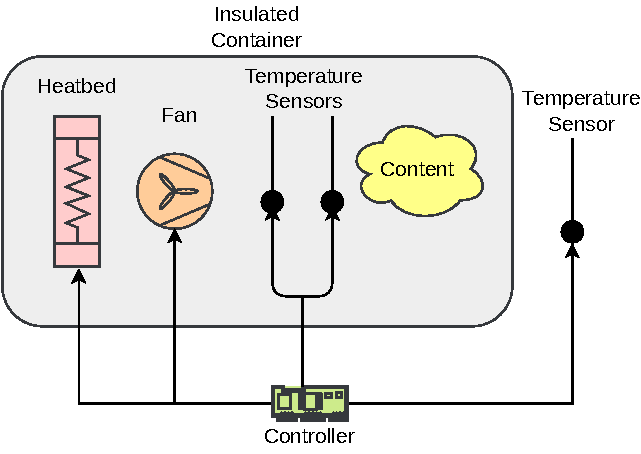
\includegraphics[width=\textwidth]{images/system_hardware.pdf}
		\caption{Hardware overview of the incubator.}
		\label{subfig:incubator_hw}
	\end{subfigure}%
	~
	\begin{subfigure}[t]{0.48\textwidth}
		\centering
		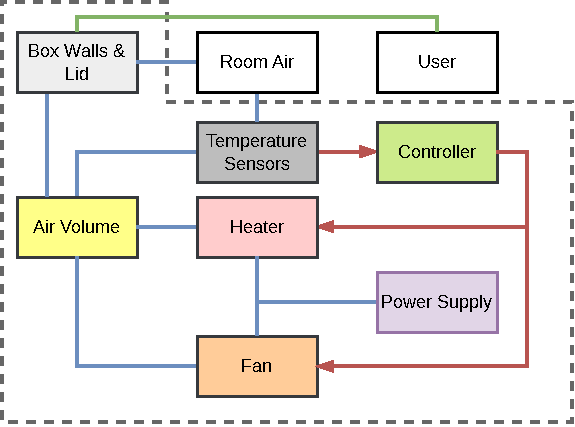
\includegraphics[width=\textwidth]{images/system_block.pdf}
		\caption{Block diagram of the incubator.}
		%The blue connections represent energy interactions, the red connections represent digital information flow, and the green connection represents the user's action by opening and closing the lid. The dashed box represents the system boundary.
		% Outcommented in-depth description of block diagram as it takes up a lot of space.
		\label{subfig:incubator_blocks}
	\end{subfigure}%

	\begin{subfigure}[t]{0.9\textwidth}
		\centering
		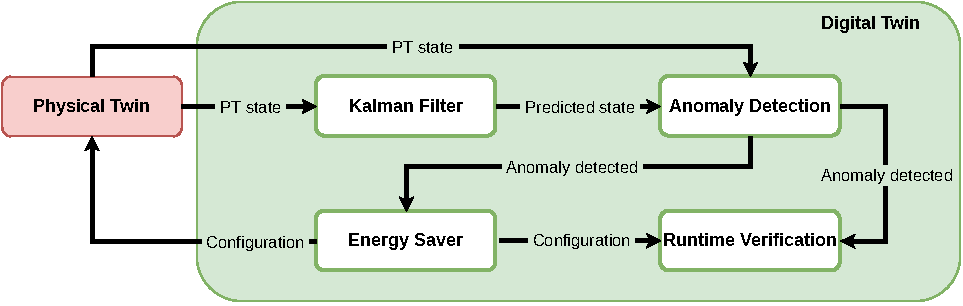
\includegraphics[width=\textwidth]{images/incubator_anomaly_HL.pdf}
		\caption{High-level overview of the DT components relevant to the examples below. Arrows indicate RabbitMQ messages and associated data.}
		\label{subfig:incubator_anomaly}
	\end{subfigure}
	\caption{Overview of the incubator.}
	\label{fig:incubator}
\end{figure}

\begin{comment}
\begin{figure}[htb]
	\centering
	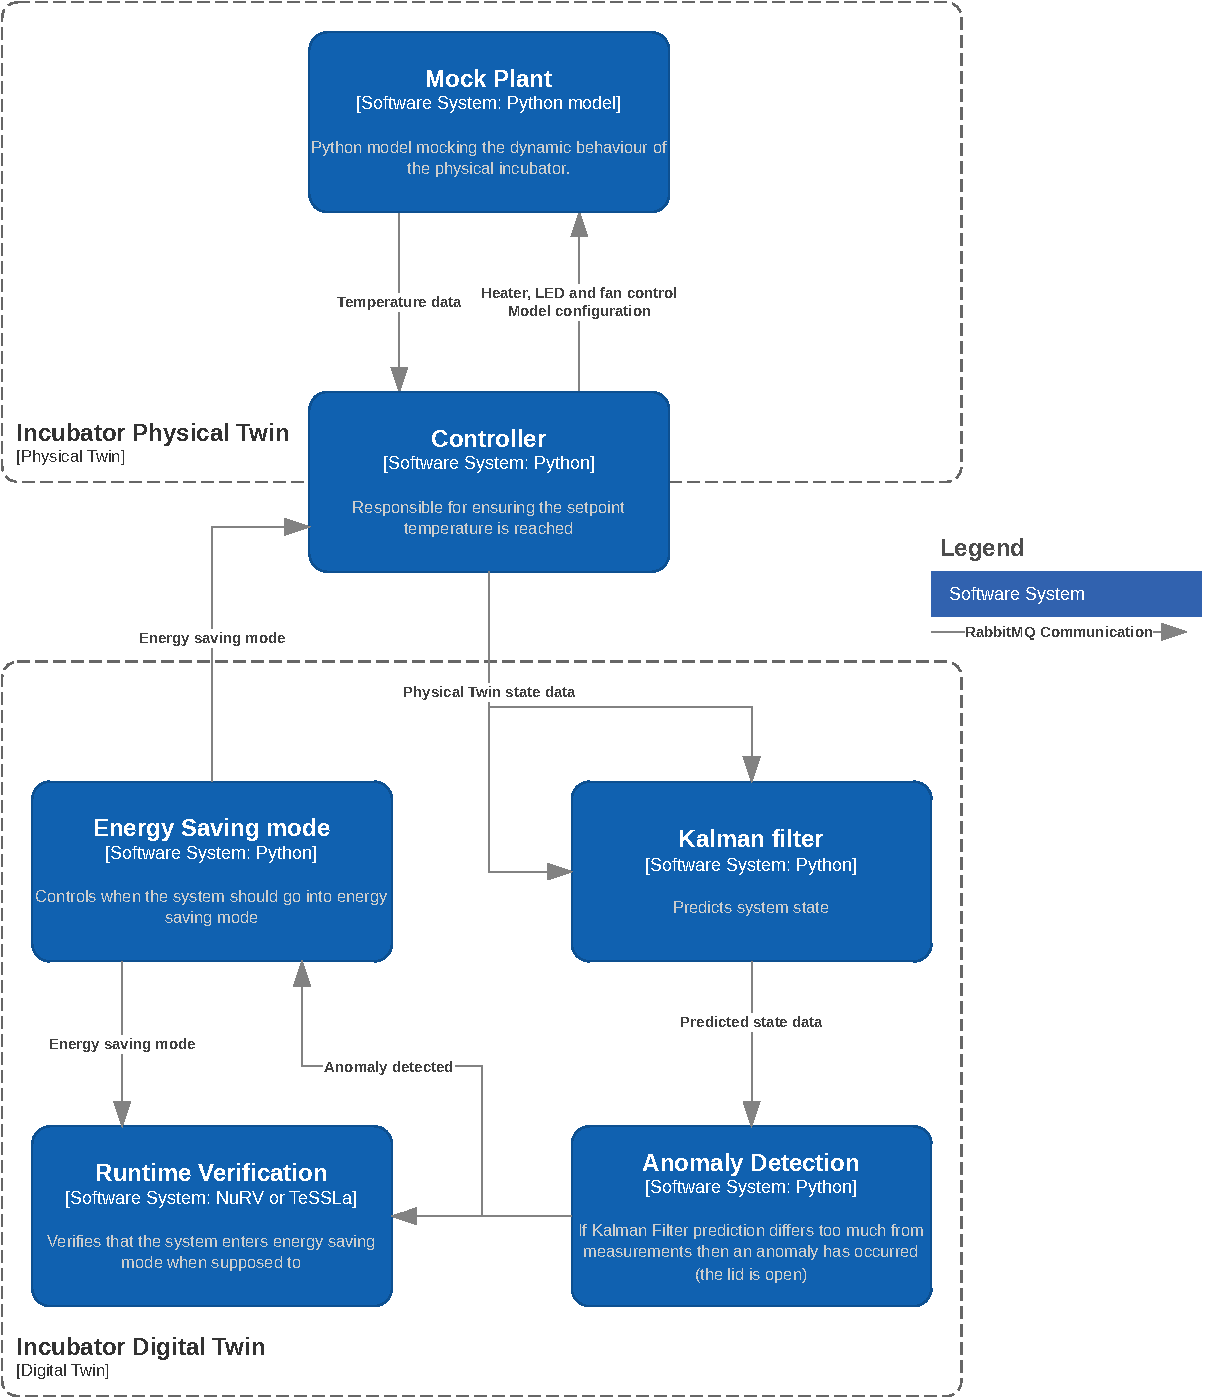
\includegraphics[width=0.9\textwidth]{images/with_energy_saving.pdf}
	\caption{Schematic overview of the incubator DT and PT interaction.}
	\label{fig:incubator}
\end{figure}
\begin{subfigure}[t]{0.48\textwidth}
	\centering
	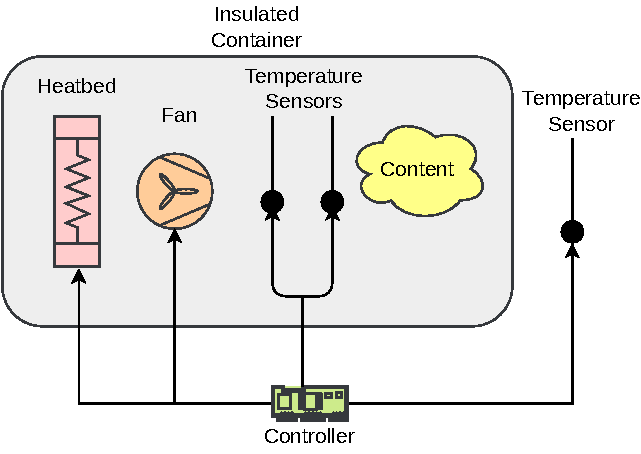
\includegraphics[width=\textwidth]{images/system_hardware.pdf}
	\caption{Hardware components of the incubator.}
	\label{subfig:incubator_hw}
\end{subfigure}%
\end{comment}
\subsection{NuRV FMU monitor}\label{subsec:NuRVmoni}
NuRV provides the capability to export runtime monitors as standalone FMU components. This feature enables users to easily interface monitors within custom applications using a variety of libraries that support the FMU standard.
This section outlines how to utilize these FMU monitors to perform an early validation of the internal components of the Incubator before its deployment. Specifically, it is shown how to validate the energy saver and anomaly detection components using an FMU monitor.

\subsubsection{Monitor definition and integration}
The monitor is defined by the SMV model seen in \cref{fig:nurv_orbit_spec}. This model specifies a safety LTL property: Whenever an anomaly occurs, the system should reconfigure itself and enter energy-saving mode within a maximum of \textinline{3} time steps. The output of this monitor can be a final verdict of either \textit{true} or \textit{false}, or \textit{unknown} if there is insufficient information to reach a definitive conclusion.

%\begin{noindent} % Do not delete
\begin{figure}[ht]
	\begin{textcode}
		MODULE main
		VAR
			anomaly : boolean;
			energy_saving : boolean;
		LTLSPEC -- Safety
			G (anomaly -> F [ 0, 3 ] energy_saving)
	\end{textcode}
	\caption{NuRV monitor model}
	\label{fig:nurv_orbit_spec}
\end{figure}%
%\end{noindent}

\subsubsection{Simulation environment}
For the validation process, a simulation environment was established
comprising several components (depicted in ~\cref{fig:nurv_fmi_simulation}): the \textit{energy saver} and \textit{anomaly detection} components, each encapsulated within distinct FMUs, along with the NuRV monitor, exported by NuRV using the specification in \cref{fig:nurv_orbit_spec}. The input data for the simulation is generated by a purpose-built FMU component named \textit{source}, which supplies testing data, simulating an anomaly occurring at time \textinline{t=60s}. A final component, \textit{watcher}, is employed to verify whether the energy saver activates in response to an anomaly reported by the anomaly detector. The FMUs for the energy saver and anomaly detector were constructed packaging their Python code using \textinline{unifmu}\footnote{\url{https://github.com/INTO-CPS-Association/unifmu}}, while the \textit{source} and \textit{watcher} components were generated using \textinline{OpenModelica}\footnote{\url{https://openmodelica.org/}}. \textinline{maestro}\footnote{\url{https://github.com/INTO-CPS-Association/maestro}} served as the co-simulation engine.%
%
\begin{figure}[ht]
	\centering
	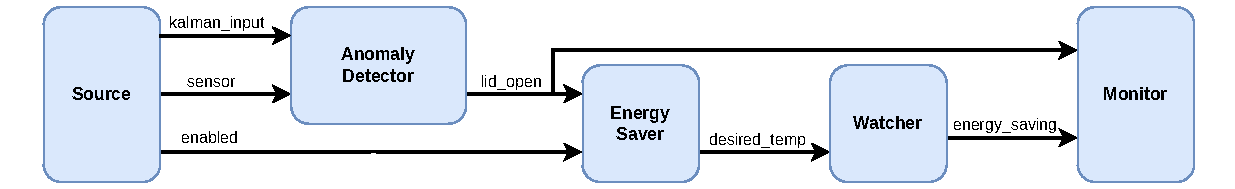
\includegraphics[width=\columnwidth]{images/FMI-communication.pdf}
	\caption{Simulation architecture of components and their exchanged signals}
	\label{fig:nurv_fmi_simulation}
\end{figure}%
%
\subsubsection{Simulation creation and execution}
The setup of the simulation is automatically performed through the \textinline{create} script, which installs the required dependencies and compiles the monitor from its specification model. The simulation is initiated using the DTaaS \textinline{execute} script, which also starts the \textit{maestro} co-simulation engine to simulate the system. Given the characteristics of the FMU monitor exported by NuRV, each invocation of the \textit{doStep} function corresponds to a logical heartbeat of the monitor. Consequently, this allows the monitor to assess the current values of its inputs and determine the appropriate outcome, thus providing validation of the system.


\subsection{NuRV FMU service monitor}\label{subsec:NuRVsermoni}
It is not possible to directly integrate the NuRV FMU monitor with the deployed Incubator.
However, by implementing straightforward wrapper logic, it becomes viable to expose the FMU as an internal service, thereby enabling its utilization within the system.
Theoretically, automating this process could be achieved through the development of a dedicated tool; however, no such tool currently exists to the authors' knowledge.
For the purposes of this tutorial, a Python-based prototype has been developed to demonstrate the potential functionality of such a tool.
It is important to underscore that this solution serves as a prototype only, and certain challenges, such as fault tolerance, remain unaddressed.%
%
\begin{figure}[ht]
	\centering
	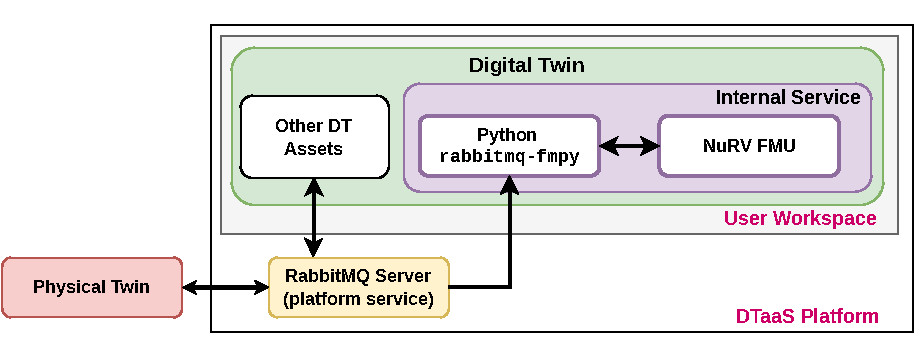
\includegraphics[width=\columnwidth]{images/NuRV-FMU-integration.pdf}
	\caption{Overview of components involved with the NuRV FMU service monitor. Notice that \textinline{rabbitmq} and \textinline{fmpy} are libraries.}
	\label{fig:nurv-fmu-service}
\end{figure}%
%
\subsubsection{Overview}
As depicted in \cref{fig:nurv-fmu-service}, the tool leverages the Python libraries \textinline{rabbitmq}\footnote{\url{https://pypi.org/project/rabbitmq/}} and \textinline{fmpy}\footnote{\url{https://pypi.org/project/FMPy/}}, to realize its functionality.
\textinline{rabbitmq} facilitates subscription to the RabbitMQ topics that are relevant for the monitor.
\textinline{fmpy} enables the simulation of an FMU within Python, allowing the introduction of custom logic between each simulation step.
In conjunction, this tool orchestrates its operations such that upon the occurrence of a new message on a RabbitMQ topic, the internal state of the Python program is updated, and the signals are subsequently forwarded to the FMU monitor, resulting in the generation of a new verdict.\\
Given the reuse of the FMU, the NuRV specification remains identical to the one outlined previously.

\subsubsection{Creation, execution, and termination}
As an extension of the configuration provided in \cref{subsec:NuRVmoni}, the prerequisites are a superset of those previously outlined.
Additionally, the Python libraries \textinline{fmpy} and \textinline{rabbitmq} must be installed.
As a consequence, the \textinline{create} script fulfills the same function as described above, while also installing the requisite additional Python libraries.\\
In this configuration of the Incubator, an additional service in the form of the RV monitor is initiated concurrently with the DT.
Given that the monitor is deployed as an internal service, it becomes the responsibility of the DT to manage the monitor, thereby intertwining their lifecycles.
Consequently, the \textinline{execute} script commences the DT as usual but with the inclusion of starting the monitor.
This enables the continuous monitoring of the anomaly detection and energy saving blocks, facilitating their verification at runtime.

\subsection{NuRV ORBit2 monitor}\label{subsec:NuRVORBIT}
% Native DTaaS integration of monitors with orbit
Alternatively, NuRV can also be deployed as a standalone monitoring server service accessible to the DT.
Consequently, the NuRV monitor and DT operate independently with their lifecycles entirely decoupled.
This section delineates the steps to achieve this with the incubator.

\subsubsection{NuRV monitor server}
NuRV supports a network-based \textit{monitoring server} mode: from the interactive shell mode, NuRV can enter with a command into a network listening state. This enables user code to remotely execute the heartbeat command for online monitoring.
In server mode, NuRV can accommodate multiple clients connecting to multiple servers. In this context, each \textit{monitor server} refers to a running NuRV process where numerous LTL properties are incorporated alongside their respective runtime monitors, established through the \textinline{build_monitor} command. It should be emphasized that a single NuRV process has the capacity to administer multiple monitors, each tailored to different LTL properties.


\subsubsection{Monitor integration}
The process of connecting the monitor server to the DT of the incubator is automated by the \textinline{execute} script. This script, in turn, employs a Python script file, that initially launches the \textinline{omniNames} CORBA Name Service utility from the \textit{omniORB} toolset, followed by starting the \textinline{NuRV_orbit} version of NuRV. Subsequently, a connection is established with the monitor server using the \textit{omniORB} Python library. Once this connection is established, the Python script starts the incubator DT and subscribes to relevant RabbitMQ topics such as energy saver status and lid open status. The lid open status is mapped to the anomaly for the NuRV monitor.\\
\Cref{fig:nurv-orbit-architecture-diagram} shows the architecture of the system comprising the incubator DT and the NuRV monitoring server.%
%
\begin{figure}[ht]
	\centering
	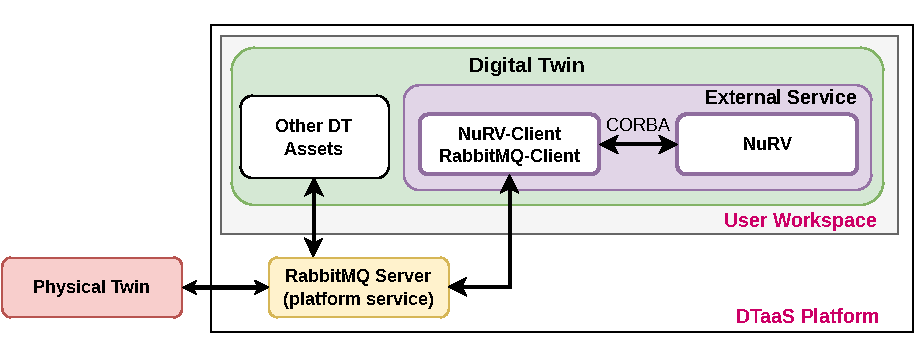
\includegraphics[width=\columnwidth]{images/NuRV-native-integration.pdf}
	\caption{Overview of components involved with the NuRV ORBit2 monitor.}
	\label{fig:nurv-orbit-architecture-diagram}
\end{figure}
%
Upon receiving a message, the DT's status is relayed to NuRV via a heartbeat operation call through the CORBA interface. NuRV responds to this heartbeat by providing the monitor's output. If the monitor's output represents a final verdict, the monitor is reset to prepare for its utilisation for the subsequent execution of the DT.


%------------------------------------------------------------------------------------------------------------------
\subsection{TeSSLa passive monitor}\label{subsec:TESLA1}
%\prasad{can this example be written as external monitor? The example can be made into external monitor by separating the execute and terminate scripts of DT and Telegraf+connector+TeSSLA block. The work can be done after the submission but might be manageable. Apologies to Lars/Hannes if the estimation of work required is substantial. Their feedback needs to be taken before making a final decision.}
%\morten{@prasad: Talked to Lars about this. He agreed.}
%This subsection describes the integration of a TeSSLa-based monitoring system as an internal service in the incubator's DT on the DTaaS platform.
%It serves two purposes: reporting on the system status as an external monitor (passive monitor) or directly controlling a part (active monitor). Both options are described in the following subsections.
%\morten{Streamlined subsection/subsubsection structure. Removed intro text (now included in section 4.0)}

As an alternative to NuRV, the RV tool TeSSLa can be utilized for monitoring the DT properties.
Similar to the example presented in~\cite{TT-Connector}, the monitor consists of three parts (see \cref{fig:architecture-diagram}).
At its core, the TeSSLa monitor processes input streams and produces output streams, but is not itself capable of integrating them into a larger system context.
A helper function (Connector) is compiled to handle the streams by connecting TeSSLa streams to sockets with which external tools can interact.
Telegraf provides an additional layer of flexibility by adding
\begin{itemize}
	\item reconfigurability at runtime -- the service can be configured to automatically adapt to a changing configuration file using the \textinline{--watch-config} flag, or simply restarted without losing the internal state of the monitor,
	\item data aggregation with basic statistical operations (such as count, mean, min or histograms),
	\item stream processing for filtering or transforming data streams, and
	\item by providing more than 200 integrations with different services and protocols to send or receive streams\footnote{\url{https://docs.influxdata.com/telegraf/v1/plugins/}}.
\end{itemize}%
%
\begin{figure}[tbp]
	\centering
	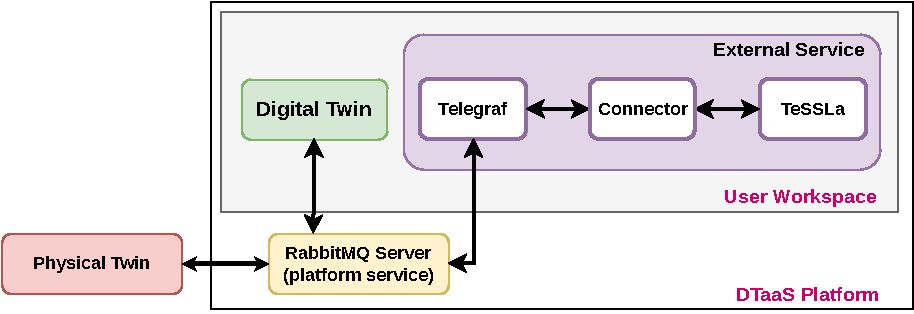
\includegraphics[width=\columnwidth]{images/TeSSLa-integration.pdf}
	\caption{Overview of components involved with the TeSSLA passive and active monitors.}
	\label{fig:architecture-diagram}
\end{figure}%
%
The \texttt{create} script prepares the system by ensuring that the necessary tools and software are installed and configured.
It installs Java, Rust and Telegraf on the system, clones the repository for the incubator DT example\footnote{\url{https://github.com/INTO-CPS-Association/example_digital-twin_incubator?tab=readme-ov-file\#running-the-digital-twin}} and downloads the necessary files for the TeSSLa-Telegraf Connector\footnote{\url{https://git.tessla.io/telegraf/tessla-telegraf-connector/-/blob/master/Release/tessla-telegraf-connector.zip}}. Two files, a TeSSLa specification and a Telegraf configuration, must be provided by the user.

A TeSSLa specification suitable for this scenario (shown in \cref{fig:tessla_spec_passive}) monitors two key states of the incubator: whether the lid is open and whether the energy saving mode is used, which are passed to the TeSSLa monitor via different event streams.
The helper function \textinline{raisingDelay} delays any change from \textinline{false} to \textinline{true} by three time steps without affecting changes from \textinline{true} to \textinline{false}.
This function is used to define an internal data stream \textinline{critical} that represents when the energy saving mode is expected to be active.
If it is not, an \textinline{alert} stream is set to \textinline{true}.
This stream is sent back to the system.
The \textinline{@TelegrafIn} and \textinline{@TelegrafOut} annotations allow the compiler to automatically create the Connector function and add to the Telegraf configuration.
%
\begin{figure}[ht]
	\begin{textcode}
		include "./Telegraf.tessla"

		@TelegrafIn("amqp_consumer","host=<hostname>", "lid_open")
		in lid_open: Events[Bool]

		@TelegrafIn("amqp_consumer","host=<hostname>", "energy_saver_on")
		in energy_saver: Events[Bool]

		def delayedOpen = raisingDelay(lid_open, 3)
		def critical = lid_open && delayedOpen
		def alert = critical && !energy_saver

		@TelegrafOut("alert")
		out alert

		def raisingDelay(e: Events[Bool], d: Int):
		Events[Bool] = merge3(false, const(true, delay(const(d, boolFilter(e)), e)), const(false, falling(e)))
	\end{textcode}
	\caption{a TeSSLa specification for the passive monitor}
	\label{fig:tessla_spec_passive}
\end{figure}%
%
The Telegraf configuration consists of two parts -- where to connect to external data sources and sinks (RabbitMQ in this case), and how to connect to the TeSSLa monitor.
The first has to be specified manually, as it changes from case to case.
Here it configures the AMQP plugin to connect to the RabbitMQ server, subscribe to the topics \textinline{incubator.diagnosis.plant.lidopen} as well as \textinline{incubator.energysaver.status} and publish the monitor verdict to the topic \textinline{incubator.energysaver.alert}.

The \texttt{execute} script uses the following command to add the configuration of how to communicate with the TeSSLa monitor to the supplied Telegraf configuration, create and run the Connector helper function, and compile as well as run the monitor.%
%
\begin{figure}[ht]
	\begin{textcode}
		./TesslaTelegrafConnector -i ./incubator.tessla -c ./telegraf.conf -r
	\end{textcode}
	\caption{Command used within execute lifecycle script.}
\end{figure}%

%
The script then starts the Telegraf service with \textinline{systemctl start telegraf}. This procedure allows data flow to and from the RabbitMQ broker, facilitating the collection, processing and monitoring of sensor data.

The \texttt{terminate} script stops the Telegraf service as well as the TeSSLa monitor and removes all temporary files.

\subsection{TeSSLa active monitor}\label{subsec:TESLA2}
To use TeSSLa as a monitor to directly control the PT, the TeSSLa specification and the Telegraf configuration must be adapted.

To adapt the TeSSLa specification to control the energy saver mode instead of monitoring, the energy saver status is no longer needed as an input and the delayed signal can be provided as an output stream to switch on the energy saver if the lid is still open. As only the rising edge is delayed, the energy saving mode is switched off as soon as the lid is closed again.

The notable change in the Telegraf configuration is the line shown in \cref{fig:telegraf_json_transformation} in the AMQP output plugin, which translates the boolean value for controlling the energy saving mode into the JSON format required by the incubator. It uses the JSONata\footnote{\url{https://jsonata.org/}} transformation style.
By adding this post-processing step to Telegraf\footnote{
	Telegraf first introduced the JSON transformation feature in version 1.24, which has not yet been widely distributed to package repositories.
}, the user is able to change the formatting or desired temperature setting in the running system by changing the configuration without recompiling the monitor or losing its internal state.%
%
\begin{figure}[ht]
	\begin{textcode}
		transform = '{"temperature_desired": fields.value ? 21 : 35}'
	\end{textcode}
	\caption{Telegraf JSON transformation}
	\label{fig:telegraf_json_transformation}
\end{figure}%














% notes for reference only –– TeSSLa spec for active mode and Telegraf conf
\iffalse



	% telegraf passive – shordened
	\begin{figure}[ht]
		\centering
		\begin{lstlisting}[style=code]
\begin{lstlisting}[style=code]
[agent]
interval = "1s"
flush_interval = "1s"
[[inputs.amqp_consumer]]
    <...>
	binding_key = "incubator.diagnosis.plant.lidopen"
	json_string_fields = ["lid_open"]
[[inputs.amqp_consumer]]
    <...>
	binding_key = "incubator.energysaver.status"
	json_string_fields = ["energy_saver_on"]
[[outputs.amqp]]
    <...>
	routing_key = "incubator.energysaver.alert"

[[outputs.socket_writer]]
  urls = ["udp://localhost:1653"]
  data_format = "influx"
[[inputs.socket_listener]]
  service_address = "udp://localhost:1654"
  data_format = "influx"
	\end{lstlisting}
		\caption{Telegraf configuration for the TeSSLa Monitor. Some fields have been dropped for brevity. See \lars{link to repository} for the complete configuration. \lars{ToDo: remove + link and explain in text}}
	\end{figure}


	% telegraf passive
	\begin{figure}[ht]
		\centering
		\begin{lstlisting}[style=code]

[agent]
interval = "1s"
flush_interval = "1s"
[[inputs.amqp_consumer]]
	brokers = ["amqp://localhost:5672"]
	username = "incubator"
	password = "incubator"
	exchange = "Incubator_AMQP"
	exchange_durability = "transient"
 	data_format = "json"
  	queue = "telegraf"
	queue_durability = "transient"
	binding_key = "incubator.diagnosis.plant.lidopen"
	json_string_fields = ["lid_open"]

[[inputs.amqp_consumer]]
    <...>
  	queue = "telegraf"
	queue_durability = "transient"
	binding_key = "incubator.energysaver.status"
	json_string_fields = ["energy_saver_on"]

[[outputs.amqp]]
    <...>
	routing_key = "incubator.energysaver.alert"
	namepass = ["alert"]

[[outputs.file]]
	files = ["stdout"]

[[outputs.influxdb]]
  urls = ["udp://localhost:1653"]

[[inputs.socket_listener]]
  service_address = "udp://localhost:1654"
  data_format = "influx"
	\end{lstlisting}
		\caption{Telegraf configuration for the TeSSLa Monitor. The redundant fields of the second AMQP consumer have been dropped for brevity.\lars{move to appendix or provide link to repository?}}
	\end{figure}

	\begin{figure}[H]
		\centering
		\begin{lstlisting}[style=code]
include "./Telegraf.tessla"

@TelegrafIn("amqp_consumer","host=<hostname>", "lid_open")
in lid_open: Events[Bool]

def delayedOpen = raisingDelay(lid_open, 3)
def result = lid_open && delayedOpen

@TelegrafOut("result")
out result
def raisingDelay(e: Events[Bool], d: Int): Events[Bool] = merge3(false, const(true, delay(const(d, boolFilter(e)), e)), const(false, falling(e)))
	\end{lstlisting}
		\caption{TeSSLa specification}
		\label{fig:tessla_spec_active}
	\end{figure}



	\begin{figure}[ht]
		\centering
		\begin{lstlisting}[style=code]
[agent]
interval = "1s"
flush_interval = "1s"

[[inputs.amqp_consumer]]
	brokers = ["amqp://localhost:5672"]
	username = "incubator"
	password = "incubator"
	exchange = "Incubator_AMQP"
	exchange_durability = "transient"
	queue = "telegraf"
	queue_durability = "transient"
	binding_key = "incubator.diagnosis.plant.lidopen"
	data_format = "json"
	json_string_fields = ["lid_open"]

[[inputs.amqp_consumer]]
	brokers = ["amqp://localhost:5672"]
	username = "incubator"
	password = "incubator"
	exchange = "Incubator_AMQP"
	exchange_durability = "transient"
	queue = "telegraf"
	queue_durability = "transient"
	binding_key = "incubator.energysaver.status"
	data_format = "json"
	json_string_fields = ["energy_saver_on"]

[[outputs.amqp]]
	brokers = ["amqp://localhost:5672"]
	username = "incubator"
	password = "incubator"
	exchange = "Incubator_AMQP"
	exchange_durability = "transient"
	routing_key = "incubator.update.closed_loop_controller.parameters"
	namepass = ["result"]
	data_format = "json"
	use_batch_format = false
    json_transformation = '{"temperature_desired" : fields.value ? 21 : 35}'


[[outputs.file]]
	files = ["stdout"]


[[outputs.influxdb]]
  urls = ["udp://127.0.0.1:1653"]
[[inputs.socket_listener]]
  service_address = "udp://:1654"
  data_format = "influx"
	\end{lstlisting}
		\caption{Telegraf configuration for the TeSSLa Monitor. The redundant fields of the second AMQP consumer have been dropped for brevity.}
		\label{fig:telegraf_conf}
	\end{figure}

\fi


%------------------------------------------------------------------------------------------------------------------

\section{Concluding remarks} \label{sec:conclude}

This tutorial paper delineates the process of integrating RV within existing AS, by demonstrating different integration patterns through five use cases.
Although the tool integrations has been demonstrated using NuRV and TeSSLa within a DT context utilizing DTaaS, the underlying concepts extend beyond these implementation details.
Consequently, the learning outcomes can be generalized, enabling tutorial participants to apply RV tools in their research to provide stronger guarantees of the correctness of their AS.
In the physical tutorial conducted at ACSOS 2024, the examples will be demonstrated sequentially, with a discussion of the deployment advantages and disadvantages of each approach.
Participants will also have the opportunity to run the examples directly on the DTaaS platform.%

\bibliographystyle{splncs04}
\bibliography{bibliographies/common.bib}

\end{document}
